\documentclass[10pt,a4paper]{article}

\usepackage[a4paper,margin=18mm,top=20mm,bottom=22mm]{geometry}
\usepackage[T1]{fontenc}
\usepackage{lmodern}
\usepackage{microtype}
\usepackage{setspace}
\usepackage{xcolor}
\usepackage{tikz}
\usetikzlibrary{arrows.meta,positioning,calc,fit,shapes.geometric,backgrounds}
\usepackage{booktabs}
\usepackage{enumitem}
\usepackage{fancyhdr}
\usepackage{hyperref}
\usepackage{caption}
\usepackage{amsmath}

\definecolor{kurrentInk}{HTML}{102326}
\definecolor{kurrentMuted}{HTML}{5F7476}
\definecolor{kurrentKaspa}{HTML}{70C7BA}
\definecolor{kurrentKaspaDark}{HTML}{2A8F86}
\definecolor{kurrentKaspaLight}{HTML}{DDF4EF}
\definecolor{kurrentPaper}{HTML}{F7FBFA}
\definecolor{kurrentLine}{HTML}{B7D8D2}
\definecolor{kurrentGold}{HTML}{B88A2A}
\definecolor{kurrentRed}{HTML}{B65353}
\colorlet{kurrentBlue}{kurrentKaspaDark}
\colorlet{kurrentTeal}{kurrentKaspa}

\hypersetup{
  colorlinks=true,
  linkcolor=kurrentKaspaDark,
  citecolor=kurrentKaspaDark,
  urlcolor=kurrentKaspaDark,
  pdftitle={Kurrent: Latest-State Settlement over Kaspa-Style Covenants},
  pdfauthor={Arthur Zhang},
  pdfsubject={Bilateral latest-state settlement channel on Kaspa, post Crescendo 10 BPS},
  pdfkeywords={Kaspa, covenants, KIP-17, KIP-20, eltoo, latest-state, contest output, MuSig2, sequence lock, settlement},
  pdfcreationdate={D:20260620T000000Z},
  pdfmoddate=\pdfcreationdate
}

\pagestyle{fancy}
\fancyhf{}
\lhead{\sffamily\small Kurrent}
\rhead{\sffamily\small Latest-State Settlement over Kaspa-Style Covenants}
\cfoot{\sffamily\small\thepage}
\renewcommand{\headrulewidth}{0.25pt}

\setlist[itemize]{leftmargin=1.35em,itemsep=0.15em,topsep=0.25em}
\setlist[enumerate]{leftmargin=1.5em,itemsep=0.15em,topsep=0.25em}
\captionsetup{font=small,labelfont={bf,sf},textfont=it}
\setstretch{1.04}

\newcommand{\term}[1]{\textsf{\textbf{#1}}}
\newcommand{\hash}{\mathsf{H}}
\newcommand{\kcell}[2]{\parbox[t]{#1}{\raggedright #2}}

\begin{document}
\color{kurrentInk}

\pagenumbering{roman}
\begin{titlepage}

\begin{tikzpicture}[remember picture,overlay]
  \fill[kurrentPaper] (current page.south west) rectangle (current page.north east);
  \fill[kurrentInk] (current page.south west) rectangle ($(current page.south east)+(0,32mm)$);
  \draw[kurrentKaspaDark,line width=1.1pt] ($(current page.west)+(18mm,36mm)$) -- ($(current page.east)+(-18mm,36mm)$);
  \node[anchor=north west,text width=155mm] at ($(current page.north west)+(18mm,-28mm)$) {
    {\sffamily\bfseries\fontsize{28}{31}\selectfont Kurrent}\\[4mm]
    {\sffamily\fontsize{16}{19}\selectfont Latest-State Settlement over Kaspa-Style Covenants}\\[9mm]
    {\large A short research note on non-confiscatory off-chain state, covenant-bound transition rules, and response-window settlement on a fast UTXO ledger.}\\[6mm]
    {\sffamily\large Arthur Zhang}
  };
  \node[anchor=south west,text=white,text width=155mm] at ($(current page.south west)+(18mm,12mm)$) {
    {\sffamily\bfseries Research note}\\[1mm]
    {\sffamily\small Contains a normative bilateral-channel specification. Prepared for technical discussion in the Kaspa ecosystem. Not a mainnet-readiness claim.}
  };
  \begin{scope}[x=1mm,y=1mm,shift={($(current page.center)+(0mm,-10mm)$)}]
    \tikzset{
      titleState/.style 2 args={
        draw=#1,
        fill=#2,
        rounded corners=4pt,
        minimum width=38mm,
        minimum height=12mm,
        line width=0.75pt,
        font=\sffamily\bfseries,
        text=kurrentInk,
        align=center
      },
      titleArrow/.style={-{Latex[length=3mm]},line width=1.05pt,kurrentKaspaDark},
      titleTag/.style={
        draw=kurrentKaspaDark,
        fill=kurrentKaspaLight,
        rounded corners=2.5pt,
        inner xsep=2.7mm,
        inner ysep=1.05mm,
        line width=0.55pt,
        font=\sffamily\scriptsize\bfseries,
        text=kurrentInk
      }
    }
    \node[font=\sffamily\small\bfseries,text=kurrentKaspaDark,align=center] at (0,39) {Basic model};
    \node[font=\sffamily\small,text=kurrentMuted,align=center,text width=132mm] at (0,33) {higher states replace lower candidates; only the survivor becomes settlement-eligible};

    \node[titleState={kurrentMuted}{white}] (s0) at (-52,17) {state $n$};
    \node[titleState={kurrentKaspaDark}{kurrentKaspaLight}] (s1) at (0,17) {state $n+1$};
    \node[titleState={kurrentKaspaDark}{kurrentKaspaLight}] (s2) at (52,17) {state $n+2$};

    \draw[titleArrow] (s0.east) -- node[above=1.7mm,font=\sffamily\scriptsize\bfseries,text=kurrentMuted,fill=kurrentPaper,inner xsep=1.8mm,inner ysep=0.5mm] {replace} (s1.west);
    \draw[titleArrow] (s1.east) -- node[above=1.7mm,font=\sffamily\scriptsize\bfseries,text=kurrentMuted,fill=kurrentPaper,inner xsep=1.8mm,inner ysep=0.5mm] {replace} (s2.west);

    \node[draw=kurrentKaspaDark,fill=kurrentInk,text=white,rounded corners=4pt,minimum width=124mm,minimum height=14mm,line width=0.75pt,font=\sffamily\bfseries] (chain) at (0,-14) {Kaspa-style covenant layer};
    \coordinate (settleIn) at ($(chain.north)+(52mm,0)$);
    \draw[-{Latex[length=3mm]},line width=1pt,kurrentKaspaDark] (s2.south) -- node[midway,right=2mm,titleTag] {settle survivor} (settleIn);
  \end{scope}
\end{tikzpicture}
\end{titlepage}
\pagenumbering{arabic}

% Document information: KIP reference snapshot, preparation date.
% The vendored KIP references (see bibliography) are pinned to the
% kaspanet/kips commit below. The statement is neutral "KIP reference
% snapshot", not a paper-edition marker; the KIP files at this commit
% are the canonical KIP content used in this paper.
% Full commit: 1aba3b8321c1d27e00b7d87bd7c74ef879efabdc
% Upstream commit date: 2026-06-02 10:59:01 -0600.
% Snapshot URL: https://github.com/kaspanet/kips/tree/1aba3b8
\newcommand{\kipsnapshot}{1aba3b8}
\begin{center}
\small
KIP reference snapshot: \texttt{kaspanet/kips@\kipsnapshot} \quad\textperiodcentered\quad
Prepared 2026-06-20.
\end{center}
\noindent{\footnotesize Any KIP text referenced in this note is the version vendored at \texttt{kaspanet/kips@\kipsnapshot}; later KIP revisions may differ.}

\section*{Abstract}

I specify a fixed-participant bilateral channel with a fixed aggregate verification key $P_{\mathrm{agg}}$, secured by a contest-output state machine over Kaspa's DAA-relative sequence maturity: a relative-sequence lock measured in DAA score. The construction is exposed to script through KIP-17 sequence introspection and the KIP-20 covenant-lineage surface. Each state update moves the channel value from a contest output of value $V$ at state $n$ to a successor contest output at state $m > n$, or to a settlement transaction after maturity.

Three primitives carry the normative bilateral channel: a fixed MuSig2 aggregate over the two participant public keys, a versioned scope identifier binding the channel's economic parameters, and a DAA-relative input sequence lock. Cooperative close is an orthogonal fast path requiring no response window; it is disjoint from the unilateral-replacement safety argument.

The safety claim is deliberately narrow. A higher authorised state has an immediately eligible covenant-preserving replacement path, while settlement of the current contest output is relatively delayed; stale-state safety is conditional on the higher replacement becoming accepted before stale settlement is accepted. The construction is non-confiscatory rather than watch-free: it removes revocation-secret forfeiture, but still depends on active monitoring and timely inclusion inside the response window. A prototype harness exercising the marker-and-verifier path is reported as evidence of model-level displacement behaviour; it does not implement the normative contest-output transaction graph.

\section{Scope}

This note specifies the normative protocol construction for a bilateral latest-state settlement channel on Kaspa, post Crescendo 10 BPS \cite{kip14}. The construction is:

\begin{itemize}
  \item Fixed-participant (two parties: $A$ and $B$);
  \item Fixed aggregate verification key $P_{\mathrm{agg}}$ (32-byte x-only BIP-340, deterministic MuSig2 over lex-sorted participant public keys);
  \item Single aggregate Schnorr signature per state certificate;
  \item Single normative state machine: $\mathrm{OpenOutput} \to \mathrm{ContestOutput}(n)$ for any valid $n$ with $0 \le n \le 2^{63}-1$, with $\mathrm{ContestOutput}(n) \to \{\mathrm{ContestOutput}(m),\ \mathrm{Settlement}(n)\}$;
  \item Two cooperative-close fast paths: $\mathrm{OpenOutput} \to \mathrm{CoopClose}$ and $\mathrm{ContestOutput}(n) \to \mathrm{CoopClose}(n)$.
\end{itemize}

Out of normative scope (relocated to dedicated sections below): marker / KIP-21 observability, factories, sum commitments, hashlock interop, zk proof systems. The prototype harness exercises the marker path; the normative specification does not depend on it. Factory material is research-only in this note: it records materialisation invariants and proof obligations, not a production compressed-commitment construction.

\paragraph{Reader map.} This note uses \emph{contest output} for the singleton channel UTXO currently under dispute. A \emph{state certificate} is the 4-tuple $(\mathsf{scope\_id}, n, \mathsf{state\_root}_n, \sigma_n)$ under the channel's fixed MuSig2 aggregate verification key, where $\sigma_n$ is an aggregate Schnorr signature over the certificate message $m_n = H_{\mathrm{KurrentStateCert/v1}}(\mathsf{scope\_id} \parallel \mathrm{le64}(n) \parallel \mathsf{state\_root}_n)$. DAA-relative maturity is relative-sequence maturity measured against the contest output's creation DAA score; the settlement branch is invalid until that score plus $\Delta$. The covenant ID is the KIP-20 lineage label carried by the channel UTXO. The marker / KIP-21 path is prototype evidence and observability infrastructure, not the bilateral fund-safety core.

\section{The Problem: Keeping an Old State Dead}

Off-chain protocols are built on a bargain. Most activity should remain local to the parties who care about it, whilst the public ledger should be invoked only for settlement, dispute, or anchoring. This bargain is attractive because it preserves the scarce resource that a base layer provides: globally agreed ordering and validation. It is also dangerous, because a locally negotiated state is not useful unless every participant can later force the correct outcome on-chain.

The hard question is therefore not how to update a balance sheet. It is how to stop an older balance sheet from coming back to life. In a channel, Alice and Bob may agree successively to states $S_0, S_1, S_2, \ldots, S_n$. State $S_i$ may have been valid when it was signed. After $S_{i+1}$ is accepted, however, $S_i$ is no longer the contract. The ledger must not be fooled by the mere history of $S_i$ having been signed.

The eltoo idea is narrow: a later authorised state should supersede an older settlement candidate by state number rather than by confiscatory revocation \cite{eltoo}. Kurrent maps that discipline onto a contest-output state machine over one relative-sequence lock and one aggregate signature. A higher valid state displaces a lower one only if the higher spend consumes the contest UTXO first; after maturity, consensus simply decides which conflicting spend it accepts. The design therefore changes the stale-state consequence, but does not remove the liveness race.

\section{From NOINPUT to Covenant-Bound Replacement}

Bitcoin eltoo realises that discipline through Bitcoin-specific transaction rebinding: NOINPUT-style floating settlement lets a later update bind to a state lineage without committing to one exact previous transaction identifier \cite{eltoo}. Perun and the virtual-state-channel line form a parallel research direction, studying multi-party virtual-channel settings in which off-chain state objects are composed and settled through formally specified channel protocols \cite{perunVSC}. Kurrent's mechanism differs from eltoo in that it does not need a Kaspa equivalent of Bitcoin's floating transaction primitive. It expresses replacement through KIP-20 covenant lineage, KIP-17 introspection, successor predicates, participant authorisation, and DAA-relative maturity. Covenant identity is an output-level lineage anchor: it identifies the continuing object, while the successor and maturity predicates decide which spends are eligible.

A Kurrent state is bound by a strict progress relation against the spent contest output. The state number $n$ lives in a state certificate
\[
  \mathsf{StateCert}_n = (\mathsf{scope\_id}, n, \mathsf{state\_root}_n, \sigma_n),
\]
where $m_n = H_{\mathrm{KurrentStateCert/v1}}(\mathsf{scope\_id} \parallel \mathrm{le64}(n) \parallel \mathsf{state\_root}_n)$ is the certificate message and $\sigma_n$ is an aggregate Schnorr signature produced by the MuSig2 protocol over $m_n$ by the fixed participant set. Participant public keys are lexicographically ordered before deterministic key aggregation. A presented successor must satisfy the same $\mathsf{scope\_id}$; a strictly higher $n$ with $n \le 2^{63}-1$; a valid certificate; principal conservation $v_A + v_B = V$; and outputs whose slots hash to the bound state root under \S\ref{sec:state-root}. The chain-extension path and the displacement path share these predicates. A displacement spend, as a higher-numbered state replacing a lower candidate, is predecessor-independent: it need not be the immediate successor of the spent state.

The design question is therefore precise: can the Kaspa covenant surface described by the KIP-17/KIP-20 direction express the required eltoo-like safety properties without a floating transaction primitive? A credible answer must show how the state-bearing output exposes its identity, how the spending transaction proves strict progress, how conservation is checked, and how the ledger environment decides whether a higher valid candidate displaced a lower one in time. Sections~\ref{sec:commitment}--\ref{sec:security} state the answer and discharge the sufficiency claim rather than assuming it.

\begin{figure}[t]
\centering
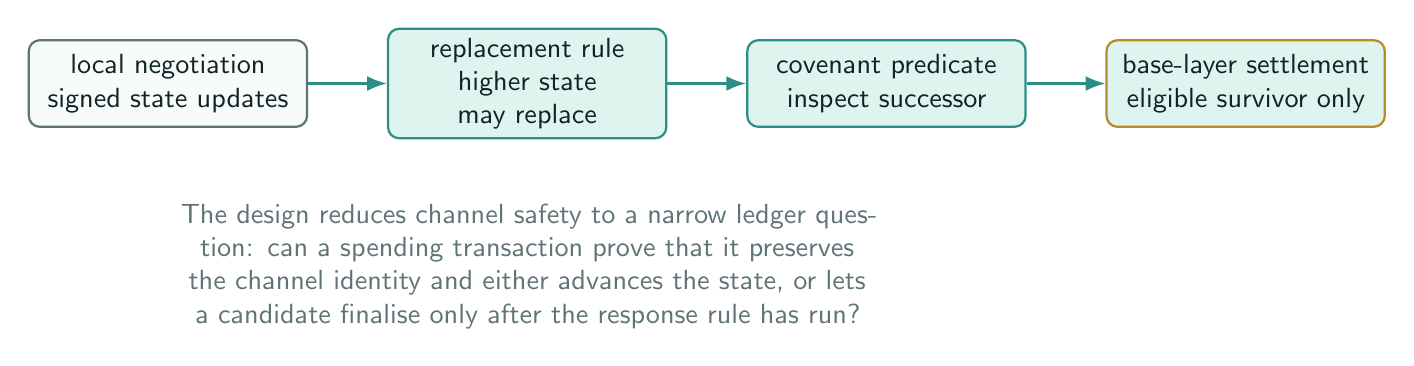
\begin{tikzpicture}[
  font=\sffamily,
  box/.style={draw=#1,fill=kurrentKaspaLight,rounded corners=4pt,minimum height=11mm,text width=33mm,align=center,thick,text=kurrentInk},
  arr/.style={-{Latex[length=2.5mm]},thick,kurrentKaspaDark}
]
  \node[box=kurrentMuted,fill=kurrentPaper] (local) {local negotiation\\signed state updates};
  \node[box=kurrentKaspaDark,right=10mm of local] (rule) {replacement rule\\higher state may replace};
  \node[box=kurrentKaspaDark,right=10mm of rule] (cov) {covenant predicate\\inspect successor};
  \node[box=kurrentGold,right=10mm of cov] (settle) {base-layer settlement\\eligible survivor only};
  \draw[arr] (local) -- (rule);
  \draw[arr] (rule) -- (cov);
  \draw[arr] (cov) -- (settle);
  \node[below=7mm of rule,text width=95mm,align=center,color=kurrentMuted] {
    \hyphenpenalty=10000\exhyphenpenalty=10000 The design reduces channel safety to a narrow ledger question: can a spending transaction prove that it preserves the channel identity and either advances the state, or lets a candidate finalise only after the response rule has run?
  };
\end{tikzpicture}
\caption{The latest-state thesis: off-chain agreement is cheap; on-chain enforcement is narrow and rule-bound.}
\label{fig:latest-state-thesis}
\end{figure}

\section{Why Kaspa-Style Covenants}

The UTXO model is deliberately austere. A coin is an output guarded by a spending condition. A transaction consumes old outputs and creates new outputs. This simplicity is one reason for the robustness of UTXO systems, but it also makes stateful protocols awkward: the state is not stored in an account; it is carried by the lineage of outputs.

Kaspa's scripting direction changes the design space. KIP-10 introduces transaction introspection opcodes, allowing a script to inspect the spending transaction's input and output counts, current input index, input and output values, and script public keys \cite{kip10}. KIP-17 extends that surface to full covenant support by adding introspection over further transaction fields, byte-string manipulation primitives, hash opcodes, and larger post-Toccata script-element limits \cite{kip17}. KIP-20 then gives covenants a first-class lineage primitive: a consensus-tracked covenant identifier carried by UTXOs and declared by outputs, so that a covenant instance has an identity that is not merely inferred from recursive witness data \cite{kip20}.

At the pinned KIP snapshot \texttt{kaspanet/kips@\kipsnapshot}, three consensus primitives carry the entire Kurrent construction: KIP-17 script introspection (sequence fields, output count, output values, output script public keys); KIP-20 covenant context (covenant identifier, authorised-output count and index, covenant-wide input and output counts); and Kaspa's DAA-relative sequence maturity, exposed through KIP-17 sequence introspection. No marker, no lane, no global ordering proof is required for bilateral fund safety. The post-Toccata partitioned sequencing surface in KIP-21 \cite{kip21} is valuable for observability, watchtower evidence, and future based-app and compressed-factory paths, but it is not a fund-safety primitive for the bilateral channel. Even though KIP-21 is present in the pinned snapshot, it remains an observability and compressed-evidence surface here, not a bilateral fund-safety requirement. A latest-state channel needs identity, inspection, transition, and the relative-sequence maturity rule; it does not need a global ordering commitment as a fund-safety gate. The broader Toccata narrative frames covenants and zk-oriented scripting as part of Kaspa's application-development trajectory \cite{kaspaBuild,toccataOutlook}.



\section{Commitment and Authorisation Model}
\label{sec:commitment}

The protocol-level commitment hierarchy splits the wire fields into three layers, each bound by a single canonical hash. The lowest-level fields are folded into a static \emph{scope identifier}; the state-dependent economic rights are folded into a \emph{state root}; the participant authorisation binds only the scope, the state number, and the state root. The result is a constant-size signed payload under a fixed participant set and a canonical commitment structure; the latter admits direct displacement without an ancestry obligation.

\subsection{Scope Identifier}
\label{sec:scope-id}

The channel is identified by a 32-byte scope identifier:
\[
  \mathsf{scope\_id} \;=\; H_{\mathrm{KurrentScope/v1}}(\mathsf{ScopeEncoding})
\]
with
\[
  \begin{aligned}
  \mathsf{ScopeEncoding} \;=\;& \mathsf{chain\_context}_{32}
   \,\|\, \mathsf{covenant\_id}_{32} \\
   & \|\, \mathsf{agg\_key}_{32}
   \,\|\, \mathrm{le32}(\Delta) \\
   & \|\, \mathrm{le16}(\mathsf{programme\_version})
   \,\|\, \mathsf{policy\_hash}_{32}
  \end{aligned}
\]
$\mathsf{chain\_context}_{32}$ binds the scope to a specific network identity (e.g., a hash of the genesis parameters), preventing a scope constructed on one chain from being replayed against the same outpoint on another chain. $\mathsf{agg\_key}_{32}$ is the 32-byte x-only BIP-340 aggregate verification key produced by deterministic MuSig2 \cite{musig2} key aggregation over lexicographically ordered participant public keys. $\mathsf{policy\_hash}_{32}$ is the v1 commitment to a canonical binary policy structure (§\ref{sec:policy}). Two-stage initialisation: $\mathsf{covenant\_id}$ is derived first via KIP-20 from the authorising outpoint and initial authorised outputs; $\mathsf{scope\_id}$ is then derived using that $\mathsf{covenant\_id}$. If the transaction carrying the authorising outpoint disappears from the accepted view during a reorganisation before it reaches the deployment's finality policy, the derived $\mathsf{covenant\_id}$ and $\mathsf{scope\_id}$ are abandoned with that view. A scope is live only if it is carried by an accepted and finalised covenant lineage in the current view; replaying a pre-reorg scope would require the same chain context, the same outpoint-derived covenant id, the same authorised outputs, the same aggregate key, and the same policy hash in a validation view where that lineage exists. Domain tags are ASCII strings used directly as BLAKE2b keyed-mode keys via the script opcode
\[
  \mathrm{OpBlake2bWithKey}(\mathrm{payload},\; \mathrm{domain\_tag}),
\]
with key length up to 64 bytes. The active hash domain tags are:
\begin{center}
\small
\texttt{KurrentScope/v1}, \texttt{KurrentState/v1}, \texttt{KurrentStateCert/v1},\\
\texttt{KurrentCoopCloseOutputs/v1}, \texttt{KurrentCoopClose/v1}.
\end{center}
A sixth tag $\texttt{KurrentPolicy/v1}$ is reserved for the policy encoding (§\ref{sec:policy}). The BLAKE2b-256 keyed mode is the standard RFC 7693 §2.5 keyed construction; BLAKE3 does not appear in the Kurrent core.

\paragraph{Canonical contest program encoding.}
The phrase ``canonical contest redeem-script preimage'' means the deterministic byte encoding
\[
  \begin{aligned}
  \mathsf{ContestScript}_n =
  \mathsf{ContestScript}(&\mathsf{programme\_version},\mathsf{chain\_context}_{32},
  P_{\mathrm{agg}},\mathsf{policy\_hash},\Delta,\\
  &n,\mathsf{state\_root}_n,\mathsf{settlement\_mask}_n)
  \end{aligned}
\]
of the v1 contest program. It includes the fixed branch structure for replacement, settlement, and cooperative close; the fixed aggregate key $P_{\mathrm{agg}}$; the committed $\Delta$; the authenticated state number $n$; the authenticated $\mathsf{state\_root}_n$; the authenticated settlement-presence mask; the domain tags above; and the exact opcode-level encodings used by the predicate. It intentionally does not embed $\mathsf{scope\_id}$, because $\mathsf{scope\_id}$ contains the KIP-20 covenant id and the genesis id itself is derived from the initial authorised-output set. Instead, every spend recomputes $\mathsf{scope\_id}$ from the input's actual introspected covenant id, the authenticated static constants, and the policy hash. The spent input's P2SH commitment authenticates the revealed $\mathsf{ContestScript}_n$; therefore $n$, $\mathsf{state\_root}_n$, and $\mathsf{settlement\_mask}_n$ are script constants, not free witness fields. A successor $\mathrm{ContestOutput}(m)$ must pay to $\mathrm{P2SH}(\mathsf{ContestScript}_m)$, where $\mathsf{ContestScript}_m$ contains authenticated $m$, $\mathsf{state\_root}_m$, and $\mathsf{settlement\_mask}_m$. Output 0's script public key is compared against that exact P2SH encoding.

\subsection{State Root}
\label{sec:state-root}

Each state $n$ binds to a 32-byte state root:
\[
  \begin{aligned}
  \mathsf{state\_root}_n \;=\; H_{\mathrm{KurrentState/v1}}\bigl(&
   \mathsf{settlement\_mask}_n \,\|\, \mathrm{le16}(\mathsf{programme\_version}) \\
   & \|\, \mathsf{0x00} \,\|\, \mathrm{commitSPK}(\mathrm{spk}_A)
    \,\|\, \mathrm{le64}(v_A) \\
   & \|\, \mathsf{0x01} \,\|\, \mathrm{commitSPK}(\mathrm{spk}_B)
    \,\|\, \mathrm{le64}(v_B) \bigr)
  \end{aligned}
\]
where
\[
  \mathrm{commitSPK}(\mathrm{spk}) \;=\; \mathrm{le16}(\mathrm{version}) \,\|\, \mathrm{le64}(\mathrm{len}(\mathrm{script})) \,\|\, \mathrm{script}.
\]
Equivalently, the state-root preimage layout is:
\begin{center}
\small
\texttt{mask || le16(programme\_version) || 0x00 || commitSPK(spk\_A) || le64(v\_A)}\\
\texttt{     || 0x01 || commitSPK(spk\_B) || le64(v\_B)}.
\end{center}
The fixed-width $\mathrm{commitSPK}$ form is the canonical commitment form used inside every signed state-root slot and inside the cooperative-close participant-output hash. It is not the byte vector returned by Toccata output introspection. Whenever the covenant compares an actual transaction output, it uses Toccata's script-public-key byte form
\[
  \mathrm{toccataSPK}(\mathrm{spk}) \;=\; \mathrm{be16}(\mathrm{version}) \,\|\, \mathrm{script},
\]
which is exactly the value pushed by $\mathrm{OpTxOutputSpk}$. For a redeem script $R$,
\[
  \mathrm{P2SH}(R) =
  \mathrm{toccataSPK}\bigl(\mathrm{ScriptPublicKey}(0,\,
  \mathrm{OpBlake2b}\,\|\,\mathrm{OpData32}\,\|\,\mathrm{BLAKE2b256}(R)\,\|\,\mathrm{OpEqual})\bigr).
\]
The conservation invariant $v_A + v_B = V$ is enforced by the covenant. Because Kaspa rejects zero-valued transaction outputs, settlement uses a canonical presence mask:
\[
  \mathsf{settlement\_mask}_n =
  \begin{cases}
  \mathsf{0x01} & v_A = 0,\ v_B = V,\\
  \mathsf{0x02} & v_A = V,\ v_B = 0,\\
  \mathsf{0x03} & v_A > 0,\ v_B > 0,\\
  \mathsf{0x00} & \text{invalid.}
  \end{cases}
\]
The mask is authenticated by both the state root and the contest script. For $\mathsf{0x03}$, settlement outputs are $A$ at index 0 and $B$ at index 1; for $\mathsf{0x02}$, the sole participant output is $A$ at index 0; for $\mathsf{0x01}$, the sole participant output is $B$ at index 0. Optional sponsor change follows the participant outputs. Replacement and opening transactions place the successor contest output at output index 0 and optional sponsor change at output index 1. No address sort is used; participant slots are positional, not lexical.

\subsection{State Certificate and Aggregate Signature}
\label{sec:state-cert}

For each state $n$:
\[
  m_n \;=\; H_{\mathrm{KurrentStateCert/v1}}
   (\mathsf{scope\_id} \,\|\, \mathrm{le64}(n) \,\|\, \mathsf{state\_root}_n)
\]
\[
  \sigma_n \;\leftarrow\; \mathrm{MuSig2Sign}
   \bigl((sk_A, sk_B),\, m_n\bigr)
\]
On-chain validity:
$\mathrm{SchnorrVerify}(P_{\mathrm{agg}}, m_n, \sigma_n) = 1$. In the Toccata opcode profile, this abstract check is realised by $\mathrm{OpCheckSigFromStack}$ over a 32-byte message hash; the raw stack values consumed are signature, message hash, and public key. The state number is constrained to $0 \le n \le 2^{63}-1$ so that $\mathrm{OpBin2Num}$ and the script arithmetic opcodes interpret it as a signed i64 without overflow; the bound is set by the script-number encoding and the full range is operationally usable, with $2^{63}-1$ itself a valid state number rather than a reserved sentinel. $\sigma_n$ is an aggregate Schnorr signature produced by MuSig2 \cite{musig2}. Participant public keys are lexicographically ordered before deterministic key aggregation, and rogue-key resistance is provided by the MuSig2 key-aggregation procedure. The signing nonce and commitment rounds remain off-chain; only the resulting aggregate $\sigma_n$ is bound on-chain. This is a liveness limitation, not a consensus ambiguity: if a participant is offline or refuses the nonce/signing round, no new state certificate is produced; the latest already-signed certificate remains the current state for the unilateral contest and settlement paths, which operate against the same contest UTXO without further authorisation from the offline party. A non-interactive emergency key, threshold fallback, or script-visible multisig alternative would be a different authorisation policy and must be committed through the policy hash; it is not an implicit runtime fallback of the fixed MuSig2 mainline.

Same-number equivocation is forbidden by signer policy, not resolved by the covenant after the fact. Each honest signer durably records the highest state number it has signed for a given $\mathsf{scope\_id}$ and signs at most one $\mathsf{state\_root}$ for that number. It signs a new certificate only for $n$ strictly greater than the recorded value. Two different roots at the same $(\mathsf{scope\_id}, n)$ cannot replace each other because neither satisfies strict progress.

\subsection{Cooperative-Close Message}
\label{sec:coop-close}

For a cooperative close over a specific input outpoint $I$ and settlement-output hash $S$:
\[
  \begin{aligned}
  S \;=\; H_{\mathrm{KurrentCoopCloseOutputs/v1}}\bigl(&
   \mathsf{settlement\_mask} \,\|\, \mathrm{commitSPK}(\mathrm{spk}_A) \,\|\, \mathrm{le64}(v_A) \\
   & \|\, \mathrm{commitSPK}(\mathrm{spk}_B) \,\|\, \mathrm{le64}(v_B)\bigr).
  \end{aligned}
\]
The authorisation message is:
\[
  m_{\mathrm{coop}} \;=\; H_{\mathrm{KurrentCoopClose/v1}}
   (\mathsf{scope\_id} \,\|\, I \,\|\, S)
\]
\[
  \sigma_{\mathrm{coop}} \;\leftarrow\; \mathrm{MuSig2Sign}
   \bigl((sk_A, sk_B),\, m_{\mathrm{coop}}\bigr)
\]
The signature binds to the exact input outpoint; it cannot be replayed against a later contest output in the same channel lineage. Cooperative close is an orthogonal fast path (§\ref{sec:state-machine}) and is disjoint from the unilateral-replacement safety argument of §\ref{sec:security}.

\subsection{Settlement Policy}
\label{sec:policy}

Although $\mathsf{policy\_hash}$ binds into $\mathsf{scope\_id}$ and therefore into the channel authorisation, the policy fields are not repeated inside $\mathsf{StateCert}_n$. They are deployment parameters that define the scope itself: a deployment that changes $\mathsf{coop\_close\_enabled}$ or selects a different $\mathsf{settlement\_shape\_id}$ produces a different $\mathsf{scope\_id}$ and is treated as a distinct channel scope.

\[
  \begin{aligned}
  \mathsf{PolicyEncoding} \;=\;& \mathrm{le16}(\mathsf{policy\_version})
   \,\|\, \mathrm{le32}(\mathsf{sponsor\_policy\_id}) \\
   & \|\, \mathrm{le32}(\mathsf{settlement\_shape\_id})
   \,\|\, \mathsf{coop\_close\_enabled}_{1}
   \,\|\, \mathrm{le32}(\mathsf{reorg\_tolerance\_daa}) \\
   \,\|\, \mathsf{reserved}_{64}
  \end{aligned}
\]
with v1 assignments: $\mathsf{policy\_version}=1$, $\mathsf{sponsor\_policy\_id}=0$ (external-sponsor-only for positive-fee protocol transactions), $\mathsf{settlement\_shape\_id}=1$ (two-party mask-bearing shape), $\mathsf{coop\_close\_enabled} \in \{0,1\}$, $\mathsf{reorg\_tolerance\_daa} \ge 1$, and $\mathsf{reserved}_{64}$ must be all-zero (rejection on non-zero is normative).
The field $\mathsf{reorg\_tolerance\_daa}$ is a deployment finality-depth commitment in DAA-score units; v1 rejects zero so that a channel scope cannot silently omit its finality policy.
\[
  \mathsf{policy\_hash} \;=\; H_{\mathrm{KurrentPolicy/v1}}(\mathsf{PolicyEncoding})
\]
When a branch needs an individual policy field, the witness supplies the canonical $\mathsf{PolicyEncoding}$ and the script recomputes $\mathsf{policy\_hash}$ before reading that field; alternatively, a production script profile may embed the fixed policy fields as constants and compare the resulting hash to the committed $\mathsf{policy\_hash}$. In either case, a branch never accepts an unbound policy field.
$\mathsf{programme\_version}$ identifies the normative protocol ABI: state encoding, certificate message, branch predicates, output shape, sequence encodings, policy encoding, numeric bounds, and verification semantics. It is bumped only when the set of valid protocol spends or the canonical bytes being signed/hashed changes. Implementation-only refactors, test harness changes, or equivalent script optimisations that preserve the protocol ABI do not bump $\mathsf{programme\_version}$; they are tracked by source commit, build profile, script hash, or deployment artefact hash.

\section{Normative Transaction State Machine}
\label{sec:state-machine}

The state machine has three branches off the long-lived contest output (unilateral replacement, unilateral settlement, cooperative close), plus an opening transition from the initial OpenOutput that produces the first ContestOutput, and a fast cooperative-close path that can also spend the OpenOutput without a response window. Cooperative close is an orthogonal fast path that is disjoint from the unilateral-replacement safety argument. Bounded transaction shapes are stated for each branch.

\begin{figure}[t]
\centering
\resizebox{0.96\linewidth}{!}{%
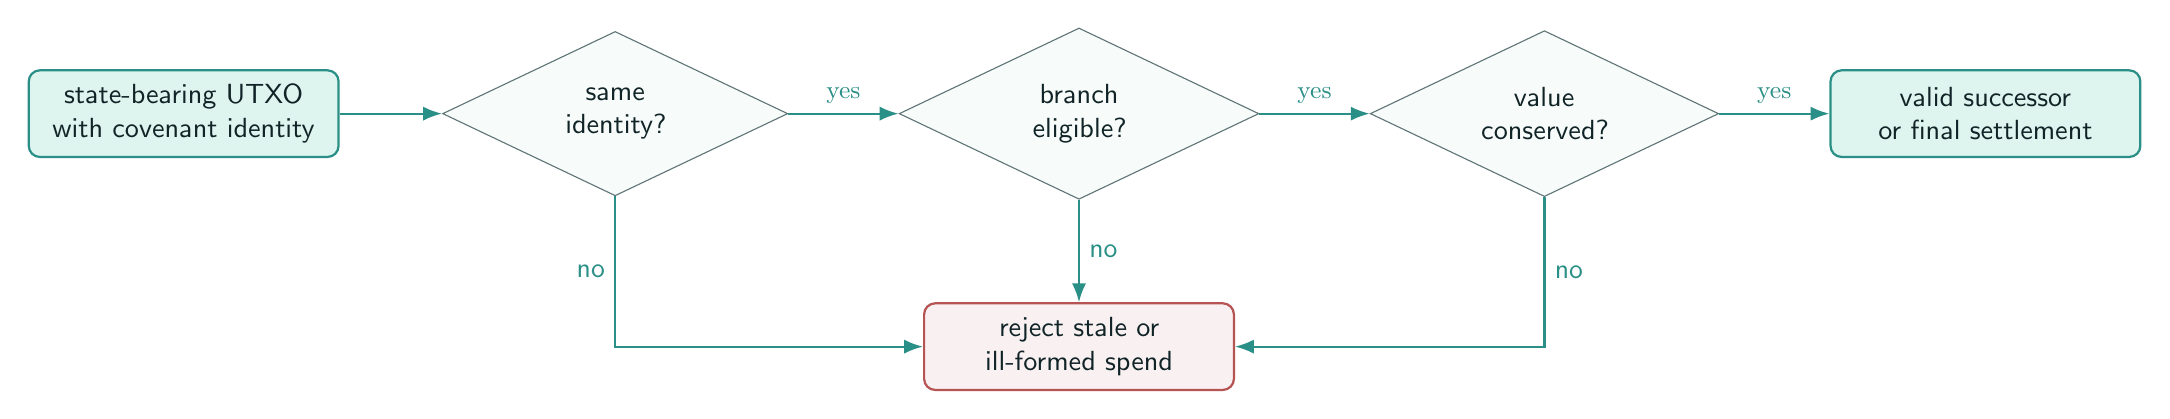
\begin{tikzpicture}[
  font=\sffamily,
  node distance=7mm,
  pred/.style={draw=#1,fill=kurrentKaspaLight,rounded corners=4pt,text width=37mm,align=center,minimum height=11mm,thick,text=kurrentInk},
  decision/.style={diamond,draw=kurrentMuted,fill=kurrentPaper,aspect=2.1,align=center,text width=27mm,inner sep=1.5pt,text=kurrentInk},
  arr/.style={-{Latex[length=2.4mm]},thick,kurrentKaspaDark}
]
  \node[pred=kurrentKaspaDark] (utxo) {state-bearing UTXO\\with covenant identity};
  \node[decision,right=13mm of utxo] (d1) {same\\identity?};
  \node[decision,right=14mm of d1] (d2) {branch\\eligible?};
  \node[decision,right=14mm of d2] (d3) {value\\conserved?};
  \node[pred=kurrentKaspaDark,right=14mm of d3] (next) {valid successor\\or final settlement};
  \node[pred=kurrentRed,fill=kurrentRed!8,below=13mm of d2] (reject) {reject stale or\\ill-formed spend};
  \draw[arr] (utxo) -- (d1);
  \draw[arr] (d1) -- node[above,font=\small] {yes} (d2);
  \draw[arr] (d2) -- node[above,font=\small] {yes} (d3);
  \draw[arr] (d3) -- node[above,font=\small] {yes} (next);
  \draw[arr] (d1) |- node[left,pos=0.25] {no} (reject);
  \draw[arr] (d2) -- node[right] {no} (reject);
  \draw[arr] (d3) |- node[right,pos=0.25] {no} (reject);
\end{tikzpicture}
}
\caption{The covenant predicate is a public, deterministic, narrow rule. Invalid spends are rejected because they fail the relevant identity, branch-eligibility, or conservation check; valid spends are replacement, settlement, or cooperative close.}
\label{fig:covenant-predicate}
\end{figure}

Figure~\ref{fig:covenant-predicate} is schematic. For replacement, branch eligibility is strict state progress $(m > n)$; for settlement, it is relative-sequence maturity; for cooperative close, it is joint authorisation bound to the exact input outpoint.

All normative protocol transactions use $\mathrm{tx.version}=\mathrm{TX\_VERSION\_TOCCATA}=1$, $\mathrm{tx.lock\_time}=0$, channel input index 0, and deterministic encodings for outpoints, sequence fields, values, and script-public-key commitments. Optional sponsor inputs, when present, are at input index 1; optional sponsor change is the last output. If no sponsor is present, the transaction input and output counts are reduced accordingly.

\subsection{Funding Genesis}
The KIP-20 genesis transaction is the base case for the singleton-lineage argument. It consumes one or more ordinary funding inputs and creates exactly one Kurrent covenant output:
\[
  \mathrm{FundingInputSet} \longrightarrow \mathrm{OpenOutput}(V).
\]
The ordered initial authorised-output set used for KIP-20 covenant-id derivation contains exactly output 0. By convention, the funding input that authorises the Kurrent covenant output is placed at input index 0; any additional funding, sponsor, or change-management inputs are placed at indices $\ge 1$. Output 0 has value $V$, declares covenant binding $(\mathsf{covenant\_id}=id,\mathsf{authorising\_input}=0)$, and pays to the canonical open script for the agreed static parameters. That open script embeds $\mathsf{chain\_context}_{32}$, $P_{\mathrm{agg}}$, $\Delta$, $\mathsf{programme\_version}$, and $\mathsf{policy\_hash}$, but not $\mathsf{scope\_id}$; when it is spent, it recomputes $\mathsf{scope\_id}$ from $\mathrm{OpInputCovenantId}(0)$ and those authenticated constants. The funding ceremony requires both participants to obtain and persist at least one valid state certificate for the intended opening state before the funding transaction is broadcast.

The funding construction rules are: the transaction has one or two outputs, output 0 is the sole Kurrent covenant output, output 0 carries covenant binding $(id,0)$, and output 0 pays to $\mathrm{P2SH}$ of the canonical open script. In Toccata, genesis covenant bindings are validated by recomputing the KIP-20 covenant id from the authorising input outpoint and the ordered authorised-output set; genesis relations are not inserted into the continuation-only $\mathrm{OpCov*}$ or $\mathrm{OpAuth*}$ script contexts. The optional second output is sponsor or ordinary change and has no Kurrent covenant binding. Genesis creates the single live Kurrent covenant UTXO; every continuation branch below preserves or terminates that singleton.

\subsection{Open Output}
The initial covenant output of value $V$ at fixed script is not spendable unilaterally; it is spendable only by:
\begin{itemize}
  \item $\mathrm{CoopClose}$ (fast path), or
  \item $\mathrm{ContestOpen}(n)$ for any valid $n$ with $0 \le n \le 2^{63}-1$.
\end{itemize}

\subsection{Contest Opening}
Spends $\mathrm{OpenOutput}$. The single covenant output is $\mathrm{ContestOutput}(n)$ for the state number $n$ authorised by the opening certificate, with value $V$ and the same covenant ID. Covenant predicates:
\begin{itemize}
  \item $\mathrm{OpCovInputCount}(id) = 1$,
  \item $\mathrm{OpCovOutputCount}(id) = 1$,
  \item $\mathrm{OpCovInputIdx}(id, 0) = i$ where $i$ is the channel-input index, so the open input is the unique covenant-authorising input for this lineage,
  \item $\mathrm{OpCovOutputIdx}(id, 0) = 0$, so the sole covenant output is at output index 0,
  \item $\mathrm{OpAuthOutputCount}(i) = 1$ for the channel input,
  \item $\mathrm{OpAuthOutputIdx}(i, 0) = 0$, so the channel input's sole authorised output is at output index 0,
  \item $\mathrm{OpOutputCovenantId}(0)=id$ and $\mathrm{OpOutputAuthorizingInput}(0)=i$, so output 0 directly declares continuation under the same covenant id and this input as its authoriser,
  \item successor output 0 has value $V$ and $\mathrm{OpTxOutputSpk}(0)=\mathrm{P2SH}(\mathsf{ContestScript}_n)$; the witness exposes the opening certificate's settlement slots $(\mathrm{spk}_A, v_A)$ and $(\mathrm{spk}_B, v_B)$, the covenant recomputes $\mathsf{state\_root}_n$ and $\mathsf{settlement\_mask}_n$ from those slots, rejects mask $\mathsf{0x00}$, and checks $v_A + v_B = V$,
  \item opening certificate $(\mathsf{scope\_id}, n, \mathsf{state\_root}_n, \sigma_n)$ validates, with $m_n$ as defined in \S\ref{sec:state-cert}:
  \[
    \mathrm{SchnorrVerify}(P_{\mathrm{agg}},\; m_n,\; \sigma_n) \;=\; 1,
  \]
  \item $0 \le n \le 2^{63}-1$ (so that the script arithmetic opcodes interpret $n$ as a signed i64 without overflow),
  \item $\mathrm{SEQ}_{\mathrm{open}} = \mathrm{le64}(2^{63})$ (disable bit set, every other bit zero).
\end{itemize}
Bounded shape:
\begin{itemize}
  \item $\mathrm{OpTxInputCount}\in\{1,2\}$ and $\mathrm{OpTxOutputCount}\in\{1,2\}$.
  \item Inputs: $[\mathrm{open\ input\ at\ idx\ }0,\ \mathrm{optional\ sponsor\ input\ at\ idx\ }1]$.
  \item Outputs: $[\mathrm{contest\ output\ of\ }V \mathrm{\ at\ idx\ }0,\ \mathrm{optional\ sponsor\ change\ at\ idx\ }1]$.
  \item Sequence: open input and sponsor input both use $\mathrm{le64}(2^{63})$ (disabled relative sequence); $\mathrm{tx.lock\_time} = 0$.
  \item Sponsor invariant: $\mathrm{sponsor\_input} = \mathrm{sponsor\_change} + \mathrm{fee}$.
\end{itemize}
The opening branch is parameterised by $n$, not fixed to $n=0$: the participants may open the channel directly at the latest state they have agreed on, including the first joint signature, without first committing to a fresh $0$-state. This avoids using a dedicated $0$-state merely to enter the contest graph, at the cost of making watchers treat the opening certificate as the first public state rather than assuming that every channel begins at $0$. Under the fixed-principal profile, the sponsor input is mandatory for any positive-fee opening by algebraic consequence of the conservation rule $v_A + v_B = V$.

\subsection{Replacement (predecessor-independent direct displacement)}
Spends $\mathrm{ContestOutput}(n)$. Produces $\mathrm{ContestOutput}(m)$ with $m > n$, $m \le 2^{63}-1$. The replacement branch is the normative path for arbitrary higher-state displacement before stale settlement is accepted: a higher-numbered valid state $m > n$ can displace a lower candidate $n$ without binding the chain of intermediate states, because the contest UTXO is the single UTXO being spent. The current local-devnet evidence path of the prototype marker harness covers adjacent-state displacement only, where each published higher candidate advances the state chain by exactly one and binds the previous commitment. The normative contest-output path does not require ancestry evidence. An ancestry-proof or intervening-chain-disclosure requirement applies only to the marker-and-verifier evidence path, where the harness records candidate history rather than consuming the contest UTXO directly; that evidence-path limitation is recorded in \texttt{KURRENT\_SECURITY\_ASSUMPTIONS.md}. Covenant predicates:
\begin{itemize}
  \item $\mathrm{OpCovInputCount}(id) = 1$,
  \item $\mathrm{OpCovOutputCount}(id) = 1$,
  \item $\mathrm{OpCovInputIdx}(id, 0) = i$ where $i$ is the channel-input index, so the channel input is the unique covenant-authorising input for this lineage,
  \item $\mathrm{OpCovOutputIdx}(id, 0) = 0$, so the sole covenant output is at output index 0,
  \item $\mathrm{OpAuthOutputCount}(i) = 1$ for the channel input,
  \item $\mathrm{OpAuthOutputIdx}(i, 0) = 0$, so the channel input's sole authorised output is at output index 0,
  \item $\mathrm{OpOutputCovenantId}(0)=id$ and $\mathrm{OpOutputAuthorizingInput}(0)=i$, so output 0 directly declares continuation under the same covenant id and this input as its authoriser,
  \item successor output 0 has value $V$ and $\mathrm{OpTxOutputSpk}(0)=\mathrm{P2SH}(\mathsf{ContestScript}_m)$; the witness exposes the successor's settlement slots $(\mathrm{spk}_A, v_A)$ and $(\mathrm{spk}_B, v_B)$, the covenant recomputes $\mathsf{state\_root}_m$ and $\mathsf{settlement\_mask}_m$ from those slots, rejects mask $\mathsf{0x00}$, and checks $v_A + v_B = V$,
  \item certificate $(\mathsf{scope\_id}, m, \mathsf{state\_root}_m, \sigma_m)$ validates,
  \item $\mathrm{SEQ}_{\mathrm{replace}} = \mathrm{le64}(2^{63})$ (disable bit set, every other bit zero).
\end{itemize}
Bounded shape:
\begin{itemize}
  \item $\mathrm{OpTxInputCount}\in\{1,2\}$ and $\mathrm{OpTxOutputCount}\in\{1,2\}$.
  \item Inputs: $[\mathrm{channel\ input\ at\ idx\ }0,\ \mathrm{optional\ sponsor\ input\ at\ idx\ }1]$.
  \item Outputs: $[\mathrm{contest\ output\ of\ }V \mathrm{\ at\ idx\ }0,\ \mathrm{optional\ sponsor\ change\ at\ idx\ }1]$.
  \item Sponsor invariant: $\mathrm{sponsor\_input} = \mathrm{sponsor\_change} + \mathrm{fee}$.
\end{itemize}
Under the fixed-principal profile, the sponsor input is mandatory for any positive-fee transaction by algebraic consequence of the conservation rule $v_A + v_B = V$.

\subsection{Settlement (unilateral, after relative-sequence maturity)}
Spends $\mathrm{ContestOutput}(n)$. Produces $\mathrm{Settlement}(n)$ using the authenticated settlement-presence mask, so that no zero-valued participant output is emitted. Covenant predicates:
\begin{itemize}
  \item $\mathrm{OpCovInputCount}(id) = 1$,
  \item $\mathrm{OpCovOutputCount}(id) = 0$,
  \item $\mathrm{OpCovInputIdx}(id, 0) = i$ where $i$ is the channel-input index, so the channel input is the unique covenant-authorising input,
  \item $\mathrm{OpAuthOutputCount}(i) = 0$ for the channel input,
  \item the revealed $\mathsf{ContestScript}_n$ authenticated by the spent input's P2SH commitment contains $n$, $\mathsf{state\_root}_n$, and $\mathsf{settlement\_mask}_n$,
  \item in the mask cases below, ``output $k$ pays $\mathrm{spk}$'' means $\mathrm{OpTxOutputSpk}(k)=\mathrm{toccataSPK}(\mathrm{spk})$,
  \item if $\mathsf{settlement\_mask}_n=\mathsf{0x03}$, output 0 pays $\mathrm{spk}_A$ with value $v_A>0$, output 1 pays $\mathrm{spk}_B$ with value $v_B>0$, and optional sponsor change is at output 2,
  \item if $\mathsf{settlement\_mask}_n=\mathsf{0x02}$, output 0 pays $\mathrm{spk}_A$ with value $V$, $v_B=0$, and optional sponsor change is at output 1,
  \item if $\mathsf{settlement\_mask}_n=\mathsf{0x01}$, output 0 pays $\mathrm{spk}_B$ with value $V$, $v_A=0$, and optional sponsor change is at output 1,
  \item $\mathsf{settlement\_mask}_n=\mathsf{0x00}$ is rejected,
  \item the covenant recomputes $\mathsf{state\_root}_n'$ from the authenticated mask, the participant SPKs, and both participant balances, then asserts $\mathsf{state\_root}_n = \mathsf{state\_root}_n'$. This binds the settlement's allocation to the state root committed by the spent contest output, so the on-chain predicate proves that each party receives the signed state's allocation rather than an arbitrary pair of values that sum to $V$,
  \item $v_A + v_B = V$ (a separate conservation predicate; the state-root recomputation above binds the allocation, but does not replace the principal-conservation check),
  \item $\mathrm{SEQ}_{\mathrm{settle}} = \mathrm{le64}(\Delta)$ (disable bit clear, bits 32--62 zero, $\Delta$ in the low 32 bits).
\end{itemize}
Bounded shape:
\begin{itemize}
  \item $\mathrm{OpTxInputCount}\in\{1,2\}$.
  \item For mask $\mathsf{0x03}$, $\mathrm{OpTxOutputCount}\in\{2,3\}$; for masks $\mathsf{0x01}$ and $\mathsf{0x02}$, $\mathrm{OpTxOutputCount}\in\{1,2\}$.
  \item Inputs: $[\mathrm{contest\ input\ at\ idx\ }0,\ \mathrm{optional\ sponsor\ input\ at\ idx\ }1]$.
  \item Outputs: canonical participant outputs selected by $\mathsf{settlement\_mask}_n$, followed by optional sponsor change.
  \item $\mathrm{tx.lock\_time} = 0$.
  \item If a sponsor input is present, the sponsor invariant $\mathrm{sponsor\_input} = \mathrm{sponsor\_change} + \mathrm{fee}$ is enforced; under the fixed-principal profile, any positive-fee settlement requires the sponsor input by the same algebraic consequence of $v_A + v_B = V$ that applies to the replacement branch.
\end{itemize}

The mandatory-sponsor rule is a deliberate fixed-principal choice, not a claim that all deployable channels must use an external fee payer. It prevents fees from silently eroding the certified participant allocation, but it introduces sponsor availability, fee-market, and single-party fee-payment dependency assumptions. A deployment that wants participants to pay fees from channel value should instead adopt a fee reserve or a principal-changing transition; both variants change the conservation predicate and belong in the committed policy hash, with principal-changing transitions treated only as a future-work sketch in §\ref{sec:future-work}.

\subsection{Cooperative Close (orthogonal fast path)}
Spends $\mathrm{OpenOutput}$ or $\mathrm{ContestOutput}(n)$. Both parties sign the same $(\mathsf{scope\_id}, I, S)$ triple where $I$ is the exact input outpoint and $S$ is the canonical hash of the participant-settlement outputs. Let
\[
  \begin{aligned}
  S \;=\; H_{\mathrm{KurrentCoopCloseOutputs/v1}}\bigl(&
  \mathsf{settlement\_mask} \,\|\, \mathrm{commitSPK}(\mathrm{spk}_A) \,\|\, \mathrm{le64}(v_A) \\
  & \|\, \mathrm{commitSPK}(\mathrm{spk}_B) \,\|\, \mathrm{le64}(v_B)\bigr)
  \end{aligned}
\]
be the canonical hash of the participant-output set under its own domain tag, and let
\[
  m_{\mathrm{coop}} \;=\; H_{\mathrm{KurrentCoopClose/v1}}(\mathsf{scope\_id} \,\|\, I \,\|\, S)
\]
as defined in \S\ref{sec:coop-close}. Covenant predicates:
\begin{itemize}
  \item $\mathsf{coop\_close\_enabled}=1$ in the authenticated policy, checked by the policy-hash binding rule of §\ref{sec:policy},
  \item $\mathrm{OpCovInputCount}(id) = 1$,
  \item $\mathrm{OpCovOutputCount}(id) = 0$,
  \item $\mathrm{OpCovInputIdx}(id, 0) = i$ where $i$ is the channel-input index,
  \item $\mathrm{OpAuthOutputCount}(i) = 0$ for the channel input,
  \item the participant outputs follow the same mask-index rule as unilateral settlement, and $\mathsf{settlement\_mask}=\mathsf{0x00}$ is rejected,
  \item the witness exposes the canonical participant-output hash $S$; the covenant recomputes $S'$ from the actual participant settlement outputs of this transaction using the formula above and asserts $S = S'$, so the cooperative-close signature is bound to the canonical participant allocation. Optional sponsor change is governed separately by the sponsor invariant and is not part of $S$,
  \item the witness exposes $\sigma_{\mathrm{coop}}$; the covenant asserts $\mathrm{SchnorrVerify}(P_{\mathrm{agg}}, m_{\mathrm{coop}}, \sigma_{\mathrm{coop}}) = 1$ with $m_{\mathrm{coop}}$ as above and $P_{\mathrm{agg}}$ the channel's fixed aggregate verification key, so the cooperative close is fully authorised by both participants under the same scope and outpoint,
  \item $v_A + v_B = V$ (a separate conservation predicate; the Schnorr authorisation binds the chosen output set, and this check ensures that the chosen set preserves the channel principal),
  \item all protocol and sponsor inputs use $\mathrm{le64}(2^{63})$ (disabled relative sequence),
  \item $\mathrm{tx.lock\_time} = 0$.
\end{itemize}
Bounded shape:
\begin{itemize}
  \item $\mathrm{OpTxInputCount}\in\{1,2\}$.
  \item For mask $\mathsf{0x03}$, $\mathrm{OpTxOutputCount}\in\{2,3\}$; for masks $\mathsf{0x01}$ and $\mathsf{0x02}$, $\mathrm{OpTxOutputCount}\in\{1,2\}$.
  \item Inputs: $[\mathrm{channel\ input\ at\ idx\ }0,\ \mathrm{optional\ sponsor\ input\ at\ idx\ }1]$.
  \item Outputs: canonical participant outputs selected by $\mathsf{settlement\_mask}$, followed by optional sponsor change.
\end{itemize}
Cooperative close is fully authorised by both parties, has no contest race, no sequence wait, and is disjoint from the unilateral-replacement safety argument of §\ref{sec:security}.

\section{Security Claims}
\label{sec:security}

This section states the security claims of the normative bilateral channel as a research note. Each claim is followed by a justification paragraph that names the predicate, UTXO, certificate, conservation, or sequence facts that discharge it. The claims are scoped to the consensus predicate and do not constitute a full formal proof; the deployment-level finality-depth assumption is stated in Claim 4, the liveness assumption is stated in \S\ref{sec:race-monitoring}, and the remaining operational obligations are recorded in \S\ref{sec:limits} and \S\ref{sec:channel-factory-scope}.

\paragraph{Claim 1 (State authentication and singleton lineage).} In any validation view reached from a valid Kurrent genesis, there is at most one live Kurrent covenant UTXO for the channel lineage. Each live contest output authenticates its own state number, state root, settlement mask, and static channel parameters through the spent input's P2SH commitment. \emph{Justification.} The funding genesis of §\ref{sec:state-machine} creates exactly one $\mathrm{OpenOutput}(V)$ and makes output 0 the only initial authorised Kurrent output. Opening and replacement consume exactly one covenant input and create exactly one authorised output at index 0; they also require $\mathrm{OpOutputCovenantId}(0)=id$ and $\mathrm{OpOutputAuthorizingInput}(0)=i$. Settlement and cooperative close consume exactly one covenant input and create zero covenant outputs. By induction, the live Kurrent lineage is singleton until it terminates. For a contest output, the revealed $\mathsf{ContestScript}_n$ is authenticated by the spent input's P2SH script public key, so $n$, $\mathsf{state\_root}_n$, and $\mathsf{settlement\_mask}_n$ are constants of the spent UTXO's script, not free witness fields. The script recomputes $\mathsf{scope\_id}$ from the actual input covenant id and the authenticated static parameters.

\paragraph{Claim 2 (Transition soundness).} Every accepted replacement of $\mathrm{ContestOutput}(n)$ creates a uniquely covenant-bound $\mathrm{ContestOutput}(m)$ with authenticated $m>n$, a valid state certificate, conserved principal, and a successor script that carries the authenticated successor state. \emph{Justification.} The replacement branch requires one covenant input, one covenant output, output 0 as the sole authorised output, direct output binding to the same covenant id and the current channel input, and $\mathrm{OpTxOutputSpk}(0)=\mathrm{P2SH}(\mathsf{ContestScript}_m)$. The successor script contains $m$, $\mathsf{state\_root}_m$, and $\mathsf{settlement\_mask}_m$. The branch checks $m>n$, verifies $\sigma_m$ over $(\mathsf{scope\_id},m,\mathsf{state\_root}_m)$, recomputes the successor root and mask from the supplied participant allocation, rejects the invalid mask, and checks $v_A+v_B=V$.

\paragraph{Claim 3 (Pre-maturity exclusion).} Settlement of $\mathrm{ContestOutput}(n)$ is invalid before the DAA-relative maturity interval expires, while a valid higher-state replacement is immediately eligible. \emph{Justification.} The settlement branch requires $\mathrm{SEQ}_{\mathrm{settle}}=\mathrm{le64}(\Delta)$ with the disable bit clear, so consensus rejects settlement until the spent contest output reaches creation DAA score plus $\Delta$ in the current validation view. The opening and replacement branches use disabled relative sequence values and do not wait on that maturity rule. The replacement must still satisfy the authenticated-state, certificate, successor-script, conservation, and singleton-lineage predicates of Claim 2.

\paragraph{Claim 4 (Conditional stale-state safety and finality).} If an honest party holds a valid certificate for $m>n$ and a replacement transaction satisfying Claim 2 becomes accepted before a stale settlement of $\mathrm{ContestOutput}(n)$ becomes accepted, then no descendant view that preserves that accepted replacement can settle the allocation committed by $\mathrm{ContestOutput}(n)$. Once that replacement reaches the deployment's Kaspa finality policy, the exclusion holds in every finality-respecting descendant view, except under violation of the underlying consensus-finality assumption. \emph{Justification.} This is the actual stale-state theorem: the later state wins only if its replacement spend is accepted first. After that acceptance, ordinary UTXO uniqueness removes $\mathrm{ContestOutput}(n)$ from the accepted UTXO set, so a later settlement of the same input is a duplicate-input spend against a spent output. The finality policy is Kaspa-native: a deployment may express it as a DAA-score, blue-score, or selected-parent/finality-depth rule defined by the target network profile, not as a Bitcoin-style ``$k$ confirmations'' rule. The protocol provides no state-number priority after maturity; if stale settlement is accepted first, the higher certificate alone cannot reverse that accepted spend.

\paragraph{Claim 5 (Settlement allocation and zero-output soundness).} Every accepted unilateral settlement pays exactly the participant allocation authenticated by the spent contest output, without requiring zero-valued transaction outputs. \emph{Justification.} The settlement branch takes $n$, $\mathsf{state\_root}_n$, and $\mathsf{settlement\_mask}_n$ from the P2SH-authenticated $\mathsf{ContestScript}_n$. It reconstructs the participant output set selected by the mask, rejects mask $\mathsf{0x00}$, rejects any mask inconsistent with $(v_A,v_B)$, recomputes $\mathsf{state\_root}_n'$ from the mask, SPKs, and balances, and asserts equality with $\mathsf{state\_root}_n$. The conservation check $v_A+v_B=V$ is separate. Masks $\mathsf{0x01}$ and $\mathsf{0x02}$ encode all-to-one terminal states with only one participant output, avoiding the consensus-invalid zero-output case.

\paragraph{Claim 6 (Cooperative-close non-interference).} Cooperative close is fully authorised by both parties and binds to the exact input outpoint. It lies outside the unilateral stale-state claim and cannot be replayed to close a later contest output. \emph{Justification.} The cooperative-close message $m_{\mathrm{coop}} = H_{\mathrm{KurrentCoopClose/v1}}(\mathsf{scope\_id} \,\|\, I \,\|\, S)$ from \S\ref{sec:coop-close} binds the input outpoint $I$ as one of its three bound fields. The Schnorr check
\[
  \mathrm{SchnorrVerify}(P_{\mathrm{agg}},\; m_{\mathrm{coop}},\; \sigma_{\mathrm{coop}}) \;=\; 1
\]
is a covenant predicate of the cooperative-close branch. A later contest output in the same channel lineage has a different outpoint $I' \neq I$, so the same signed $m_{\mathrm{coop}}$ fails the Schnorr check when the witness presents $I'$ as the spent outpoint. The cooperative-close branch is outside the unilateral-replacement claim. When it closes a $\mathrm{ContestOutput}(n)$, it consumes that contest input by joint authorisation and produces settlement outputs directly; it does not create a successor contest output and cannot be replayed against a later outpoint.



\section{Race and Monitoring Model}
\label{sec:race-monitoring}

The protocol predicate is stated in DAA-space:
\[
  a_{\mathrm{replace}} \;<\; a_n + \Delta
\]
where $a_{\mathrm{replace}}$ is the DAA score at which the replacement spend of $C_n$ becomes accepted, and $a_n$ is the DAA score of $C_n$'s creation.

Equivalently, the replacement interval is half-open: $[a_n, a_n+\Delta)$. A replacement accepted at exactly $a_n+\Delta$ is outside the response window, and settlement maturity is evaluated in the current validation view as $a_{\mathrm{current}} \ge a_n+\Delta$.

The scores are interpreted inside a particular validation view. If a reorganisation removes $C_n$, the channel is evaluated against the surviving lineage rather than against the abandoned timer. If a reorganisation removes a replacement before that replacement reaches the deployment's finality policy, the safety statement is evaluated against the surviving UTXO set; the monitor should re-evaluate the channel against that view and, if needed, publish a replacement or settlement transaction within that view's response window. Frequent reorganisations therefore increase the liveness and fee budget beyond the steady-state inclusion assumption; deployments that anticipate non-trivial reorganisation depth should record that tolerance in the channel's $\mathsf{policy\_hash}$ alongside $\Delta$. Once a replacement reaches the chosen finality policy, Claim~4 applies. The response-window state machine is reorg-aware under accepted-view UTXO semantics: timers and spends are facts of the current accepted view until finality fixes them under the deployment assumption.

After relative-sequence maturity, both the settlement transaction and a higher-state replacement may be individually valid conflicting spends of the same contest UTXO. The covenant cannot guarantee that the higher state wins merely because its state number is larger; whichever conflicting spend consensus accepts first consumes the UTXO. The protocol therefore provides no state-number priority after maturity. A higher-state replacement must be accepted before the stale settlement is accepted, full stop. The equal-DAA tie-breaker question does not arise as a channel-level rule.

Wall-clock latency is a deployment-level operational assumption:
\[
  \Pr\!\bigl[T_{\mathrm{detect}} + T_{\mathrm{construct}} + T_{\mathrm{propagate}} + T_{\mathrm{include}} < T_{\Delta}\bigr]
   \;\ge\; 1 - \varepsilon
\]
Here $T_{\Delta}$ is the expected wall-clock duration of the DAA-score interval $\Delta$ at the target network profile, with stated confidence. As a deployment-level example, the post-Crescendo Kaspa target of \mbox{10 BPS} (one block every $0.1$\,s) gives $T_{\Delta} \approx 0.1\,s \cdot \Delta$. A conservative $\Delta = 600$ DAA scores therefore corresponds to roughly a $60$\,s replacement window; a tighter $\Delta = 60$ corresponds to roughly $6$\,s. The protocol does not pick a $\Delta$ here; the deployment chooses it, and the operational confidence $\varepsilon$ is a deployment-level artefact, not a consensus-level parameter.

Publication is insufficient: the replacement must not merely be signed and broadcast. Mempool acceptance is insufficient: a transaction in the mempool is not yet a spent UTXO. Watchtower observation is insufficient: an observed transaction may be censored, replaced, or evicted. The replacement must become an accepted spend before the stale settlement does. Censorship, reorganisation, fee-market dynamics, and watchtower economics are deployment-level concerns that the consensus predicate does not solve cryptographically; the protocol separates the consensus predicate $a_{\mathrm{replace}} < a_n + \Delta$ from the deployment-level probabilistic assumption $\Pr[\cdot] \ge 1 - \varepsilon$ and treats them as distinct obligations.
The corresponding operational assumptions are recorded in
\texttt{docs/KURRENT\_SECURITY\_ASSUMPTIONS.md}; that file is part of the
security-review input and must be read together with this section.

\section{Factories as Compression of Many Channels}
\label{sec:factory}

This section is research-only. It records the invariants a future compressed factory must satisfy; it is not an implemented production factory and it is not part of the bilateral channel's normative safety claim.

A channel factory \cite{channelFactories} generalises the channel idea. Instead of placing one bilateral channel directly on-chain, several virtual channels are represented inside a shared covenant state. The base layer sees a compact factory state; the participants see many internal relationships. The attraction is obvious: one on-chain object can support many off-chain relationships.

The risk is equally obvious. Compression must not blur ownership. If one virtual channel is materialised out of the factory, the untouched channels must remain exactly what they were. A factory therefore adds a second invariant on top of latest-state replacement:

\[
  \text{factory principal}
  =
  \sum_{\text{active virtual channels}} \text{virtual principal}.
\]

This is not merely an off-chain accounting equation. Under the chosen factory representation, the equality must be cryptographically checkable. A Merkle-sum style commitment, an aggregate commitment, a proof-carrying materialisation path, or an equivalent committed internal representation can serve that role; a plain membership root does not prove principal conservation unless sums are also committed or otherwise verified.

Materialisation is sound only if it preserves that equality. The touched channel exits; its value is paid or moved according to the materialisation rule; every untouched channel remains byte-for-byte the same; the factory's remaining principal is reduced by exactly the touched principal. The conservation rule is less elegant than the state-number rule but no less central. Without conservation, a factory is not compression; it is ambiguity.

Factory non-interference is not guaranteed by the conservation equality alone. The materialisation path must carry enough committed state and proof material to show that the touched virtual channel exits under its rule, the remaining factory principal is reduced by exactly the touched principal, no new virtual claims are injected, and every untouched virtual channel remains identical under the committed representation. These are implementation audit targets, not decorative accounting rules.

This note focuses on materialisation safety: how a touched virtual channel exits without corrupting untouched virtual channels. Kurrent's paper-level factory claim is limited to materialisation invariants and proof obligations. A complete factory design must also specify the update protocol by which virtual channel updates alter the committed factory state. That includes the internal representation, which parties authorise each update, and how the next aggregate or factory commitment is produced. If the factory uses a compressed representation, non-interference must be proved through committed state and proof material, not asserted through accounting equations.

\paragraph{Scope of the present evidence.} The current local-devnet factory evidence uses a full-state typed model in which every virtual channel and the total principal are recomputed by the verifier against a complete materialisation plan. This is a bounded local-devnet evidence path for materialisation invariants: it demonstrates the structure of the model-level guarantees the compressed factory has to discharge explicitly, but it is not yet a production compressed Merkle-sum or aggregate-commitment factory. A production deployment must replace the full-state recomputation with a Merkle-sum style or equivalent committed internal representation, so that materialisation carries a proof against the factory's public commitment rather than depending on the verifier having the full pre-state. That is a separate design slice and is out of scope for the present research note.

The factory principle is therefore a natural companion to covenant identifiers. The covenant lineage says that the factory remains the same public object. The materialisation rule says what may be removed from it. The preservation rule says what must not be touched. Together they let a complex off-chain object present a simple on-chain boundary.

\section{Future Work}
\label{sec:future-work}

The normative construction in §\ref{sec:commitment}--§\ref{sec:state-machine} is intentionally narrow. The following items are required for a complete production protocol but are out of the present normative scope; they are listed here so that the boundary between the spec and the production gate is visible.

\paragraph{Hashlock interop.} Both legs share the same payment hash $h = H(r)$, and redemption on either leg reveals the same preimage $r$. Each local claim binds that shared hash to its own amount, expiry, direction, and keys. This note does not specify Lightning route-hop, PTLC, or adaptor-signature integration; those are separate protocol surfaces that build on top of the same witness-scoping discipline.

\paragraph{Key rotation and quorum changes.} The fixed-participant bilateral channel of §\ref{sec:commitment}--§\ref{sec:state-machine} is the production mainline. Rotating the participant key set, supporting $m$-of-$n$ thresholds with $n > 2$, or any participant-set transition would require an $\mathsf{EpochTransitionCertificate}$ or equivalent, with its own commitment hierarchy. The extension is in scope for a future protocol specification and is not part of the present channel mainline.

\paragraph{Factories and sum commitments.} A channel factory compresses multiple bilateral relationships behind one on-chain object. Factory materialisation safety is the principal conservation
\[
  \text{factory principal} \;=\; \sum_{\text{active virtual channels}} \text{virtual principal}
\]
discharged by a Merkle-sum style commitment, an aggregate commitment, a proof-carrying materialisation path, or an equivalent. Factories are out of the bilateral core; the design considerations are recorded in §\ref{sec:factory} and the design note \texttt{KURRENT\_FACTORY\_COMMITMENT\_DESIGN.md}.

\paragraph{KIP-21 observability and proof systems.} The post-Toccata partitioned sequencing surface is valuable for watchtower evidence, application-local proving, and future based-app and zk proof paths. It is not a fund-safety primitive for the bilateral channel, but a production deployment that needs monitoring or compressed evidence will benefit from integrating it as an observability layer. The contest-output transaction graph and the marker / KIP-21 accepted-ordering surface play complementary roles. The contest UTXO, the authenticated state carrier, the singleton-lineage predicates, and the relative-sequence maturity rule discharge the bilateral fund-safety argument of §\ref{sec:security}; no marker, lane, or accepted-ordering proof is required for that conditional stale-state theorem. The marker / KIP-21 path is the substrate for the prototype harness of §\ref{sec:channel-factory-scope} and the optional evidence layer for the based-app, compressed-factory, and zk-proof compositions above. A lane-local accepted-ordering commitment is useful where the protocol needs compact event history, portable proof objects, or watchtower observations, rather than merely a valid conflicting spend.

\paragraph{Normative contest-graph implementation.} The contest-output transaction graph specified in §\ref{sec:state-machine} is the production mainline; the local-devnet harness exercises a marker-and-verifier path as prototype evidence. A production-grade implementation of the normative contest graph, with full script bytecode, runtime cost model, and consensus-fee economics, is the next milestone beyond the present research note.

\paragraph{Principal-changing and factory extension surfaces (\textbf{sketch}).} The bilateral core of §\ref{sec:commitment}--§\ref{sec:state-machine} fixes the channel principal $V$ and the fixed-participant set; the following two extensions are forward hooks only and are not normative predicates. \emph{Principal-changing transitions.} A splice-in or splice-out would be a new authorised transition type, replacing $\mathrm{ContestOutput}(n, V)$ with $\mathrm{ContestOutput}(m, V')$ under the same $\mathsf{scope\_id}$ and a valid aggregate authorisation. The successor $\mathsf{state\_root}$ would commit to participant slots summing to $V'$, and the covenant would check that the successor contest output also has value $V'$. The stale-state exclusion argument of §\ref{sec:security} is unchanged; only the conservation predicate changes. \emph{Factory transitions.} A compressed factory would wrap the bilateral contest-output channel as a materialisable virtual leaf, consuming a $\mathrm{FactoryOutput}(\mathsf{root}, \mathsf{total})$, proving membership and principal of a touched virtual channel, and creating a successor $\mathrm{FactoryOutput}(\mathsf{root}', \mathsf{total} - V)$ whose untouched leaves are preserved under a Merkle-sum or equivalent commitment. The bilateral channel safety claim of §\ref{sec:security} applies only after materialisation; the factory safety claim is separate and must additionally prove sum conservation and untouched-leaf non-interference. Both extensions are sketched here, not specified; see \texttt{KURRENT\_FACTORY\_COMMITMENT\_DESIGN.md} for the current boundary between the implemented materialisation model and the future compressed factory commitment, and the production kernel remains the fixed-principal, fixed-participant bilateral channel.

\paragraph{Multi-participant generalisation.} The contest-output kernel is also neutral to the participant count. The same construction generalises from a bilateral $2$-of-$2$ channel to a fixed $k$-participant $k$-of-$k$ channel by replacing the two participant slots with a canonical participant vector, replacing $v_A + v_B = V$ with $\sum_{i=0}^{k-1} v_i = V$, and deriving $P_{\mathrm{agg}}$ from the ordered participant public-key list. The stale-state argument of §\ref{sec:security} is structurally unchanged: a higher-numbered valid replacement must satisfy the authenticated-state, singleton-lineage, conservation, and response-window predicates, and must be accepted before stale settlement. Threshold $t$-of-$k$ authorisation, participant-set changes, and key rotation require an explicit authorisation-policy layer or $\mathsf{EpochTransitionCertificate}$ and are treated as separate extensions.

\paragraph{Forward reference: compressed factory verification path.} When the factory evidence path eventually moves from full-state model verification to a compressed commitment, the natural on-chain verification layer for the materialisation transition is a KIP-16 wrapper \cite{kip16}. The Merkle-sum or equivalent commitment records the factory's internal asset structure; a KIP-16 proof is designed to turn the model-level factory findings (overclaimable touched leaves, injectable after-state channels, unenforced principal sum, untouched-leaf interference) into explicit proof obligations rather than into per-leaf recomputation; and the covenant script is designed to bind the proof's public inputs to the actual spent factory output, the successor output, the current factory identity, the covenant lineage, and the settlement output hash, so that a valid proof for a different factory or a different transition cannot be replayed. The combination is a bounded on-chain proof verification path: KIP-16 verifies the computation, the covenant script binds the computation to the transaction, and the Merkle-sum root is the structure the computation is over. This paragraph is a forward reference, not a current claim. It is not part of the production-readiness gate for the normative bilateral channel; it is not part of the current marker evidence mainline; and \texttt{KURRENT\_FACTORY\_COMMITMENT\_DESIGN.md} records the present boundary while the carrier for the factory root, the choice of proof system, the KIP-16 cost and pricing model, the third-party dependency model, and the security assumptions remain future compressed-factory implementation work.

\section{Eligibility, Not Retaliation}

The non-confiscatory claim is best stated as an eligibility rule. The covenant does not classify the publisher's behaviour. It classifies the candidate: same $\mathsf{scope\_id}$, authenticated contest state, strictly higher state number for replacement, valid certificate, conserved value, valid settlement mask, and response-window survival. If those checks fail, the candidate is not entitled to final settlement. This removes confiscatory revocation from the protocol logic, but it does not remove deterrence or liveness pressure entirely: the stale publisher can no longer enforce the stale settlement if a higher authorised spend is accepted in time, and honest parties still need monitoring capacity to make that happen. Claims 1--6 of §\ref{sec:security} together discharge that classification: Claim 1 authenticates the state carrier and singleton lineage, Claim 2 gives transition soundness, Claim 3 gives pre-maturity exclusion, Claim 4 states the conditional stale-state theorem and finality corollary, Claim 5 binds settlement allocation without zero-valued outputs, and Claim 6 handles the cooperative-close fast path.

This matters because a Kaspa-shaped construction has to make the replacement decision public without importing Bitcoin's floating transaction mechanism. The candidate that wins is not the one with the most sympathetic history, the largest sponsor fee, or the most convenient indexer trace. It is the one that satisfies the named eligibility rule and is accepted first by consensus. The shift is in the consequence: the response path presents the later valid entitlement, rather than a revocation secret that confiscates the stale publisher's funds.

The design still needs active monitoring. A participant, delegate, or watchtower must surface the higher authorised state before the response window closes. The response window is the liveness interval in which the higher state must become an accepted spend; the liveness proposition of §\ref{sec:security} is a deployment-level operational assumption about how likely the interval is to be satisfied under realistic propagation, censorship, and reorganisation conditions.

\section{Limitations and Open Questions}
\label{sec:limits}

The bilateral safety core specified in §\ref{sec:commitment}--§\ref{sec:state-machine} is now stated as a consensus-level predicate: the P2SH-authenticated state carrier, the KIP-20 singleton-lineage base case, the covenant successor predicate, the relative-sequence maturity rule, the MuSig2 aggregate authorisation, the settlement mask, and the cardinality checks together give the conditional stale-state safety statement of Claim~4. The fund-safety primitive does not require a consensus-recognised accepted-ordering surface.

What is not yet a complete production system is the operational layer: liveness under realistic propagation, censorship, fee-market, and reorganisation conditions, plus the wider protocol surface (factories, key rotation, hashlock interop, monitoring substrate). Production readiness for the bilateral channel additionally requires deployment-level parameterisation of the response window and finality depth; the production fee-market and sponsor policy; watchtower or monitoring architecture with a stated liveness budget; and operational key management. The post-Toccata partitioned sequencing surface is one of several valid monitoring substrates; it is not a fund-safety gate for the bilateral channel.

\paragraph{Named protocol-specification requirements (not research-note gaps).} The following items are requirements that a production protocol specification must satisfy; they are not gaps in the present research note, and are recorded here so that the boundary between the two documents is visible. \emph{(i)} The response-window state machine must specify the half-open interval $[a, d)$ semantics, the DAA-score interpretation of maturity, and the validation-view semantics at the boundary. The protocol provides no state-number priority after maturity; conflicting valid spends are resolved by ordinary consensus acceptance. \emph{(ii)} Safety must be conditional on a bounded-inclusion and fee-market assumption: an explicit fee reserve or externally attachable sponsor path; an anchor/child or package-publication fee-bumping mechanism; a congestion model; a censorship/inclusion assumption; and a watchtower fee budget. Without such an assumption, no finite response window is provably safe. \emph{(iii)} Same-number conflict handling must specify what ``first'' means under consensus finality --- first consensus-finalised certificate wins, safe fallback to the prior state, or explicit channel failure --- rather than treating arrival order at the verifier as authoritative. \emph{(iv)} Operational key management must specify the signing-ceremony procedure, the recovery path, and the rule under which the fixed-participant set is rotated; the present mainline fixes a single fixed-aggregate key for the channel lifetime. \emph{(v)} The factory design must add fixed-width arithmetic with explicit overflow rejection, range-constrained balances, canonical leaf ordering with unique virtual-channel identifiers, and a Merkle-sum or equivalent principal-commitment that the materialisation proof can verify against. \emph{(vi)} The hashlock interop must define the shared-secret scoping rule, the per-leg claim commitment, and the witness-binding discipline; the present note fixes only the shared-secret claim form (§\ref{sec:future-work}). \emph{(vii)} The deployment parameter set (response-window length $\Delta$, finality-depth policy, sponsor-policy id, $\mathsf{coop\_close\_enabled}$ flag) must be specified for the target network and recorded in the channel's $\mathsf{policy\_hash}$.

The conceptual claim is narrower and stronger: the bilateral safety primitive is the contest-output state machine of §\ref{sec:state-machine}. The remaining items above are deployment obligations and adjacent protocol surfaces, not bilateral-safety gaps. Eltoo supplies the replacement philosophy. Kurrent combines these into a Kaspa-native settlement model: state is negotiated locally, while settlement eligibility is granted only to the state that survives a public, monotone, covenant-bound rule.
\section{Production-Readiness Scope}
\label{sec:channel-factory-scope}

Kurrent as a research artefact contains three distinct protocol surfaces that share a covenant lineage but have different production-readiness dependencies. The normative bilateral contest-output channel specified in §\ref{sec:commitment}--§\ref{sec:state-machine} is the production mainline and has the smallest primitive footprint. The existing local-devnet harness exercises a marker-and-verifier prototype evidence path that demonstrates model-level displacement behaviour (§\ref{sec:security}) but is not the normative construction. The factory surface is a separate, more demanding protocol surface (§\ref{sec:factory}).

\paragraph{Accepted-ordering surface: who needs it?}

\begin{table}[ht]
\centering
\small
\renewcommand{\arraystretch}{1.2}
\begin{tabular}{@{}ll@{}}
\toprule
\textbf{Protocol surface} & \textbf{Accepted-ordering surface required?} \\
\midrule
Normative bilateral contest-output channel    & No \\
Prototype marker evidence path                & Yes (the harness depends on it) \\
Future compressed factory / based-app / zk    & Possibly / depends on the composition \\
\bottomrule
\end{tabular}
\caption{Accepted-ordering surface requirement by protocol surface. The normative bilateral channel of §\ref{sec:state-machine} does not require a consensus-recognised accepted-ordering surface for fund safety: the contest-UTXO exclusivity plus the covenant cardinality predicates plus the relative-sequence maturity rule are sufficient. The prototype marker evidence path requires an accepted-ordering substrate because the harness records and verifies candidates through the marker flow. A future compressed factory, based-app, or zk-proof composition may need a sequencing commitment for compressed evidence and global reconstructibility, depending on the proof system chosen.}
\label{tab:accepted-ordering}
\end{table}

The normative bilateral channel of §\ref{sec:state-machine} and the prototype marker evidence path are different artefacts. Conflating them would force the normative channel to depend on a prototype substrate, or would force the prototype to claim production-grade fund safety. Kurrent keeps them separate. The post-Toccata partitioned sequencing surface \cite{kip21} is one valid substrate for the prototype and the future-factory / based-app surfaces; the normative channel does not depend on it.

\paragraph{Production-readiness dependencies (normative bilateral channel).}
\begin{enumerate}
\item Deployment parameter set: response-window length $\Delta$ in DAA-score units, finality-depth policy, sponsor-policy id, $\mathsf{coop\_close\_enabled}$ flag.
\item Production fee-market and sponsor policy, including the rule that the lower stale settlement may pay a larger sponsor fee and still lose to the higher-state replacement accepted first by consensus.
\item Watchtower or monitoring architecture, with a stated liveness budget and the cross-participant response path.
\item Operational key management: signing ceremony, recovery path, fixed-participant set rule.
\item Independent review of the covenant bytecode, the consensus predicate, and the script-engine cost model.
\end{enumerate}

\paragraph{Production-readiness dependencies (prototype marker evidence path).}
The harness exercises lane binding, candidate evidence reconstruction, sponsor-accounting checks, and model-level displacement behaviour. It does not implement the normative contest-output transaction graph; it is the prototype evidence path. Its production-quality upgrade is a normative-graph implementation (§\ref{sec:future-work}), at which point the harness becomes a regression suite rather than the mainline.

\paragraph{Production-readiness dependencies (future compressed factory / based-app / zk).}
The factory surface requires a principal-commitment (Merkle-sum or equivalent) and a materialisation proof path. A based-app composition may use the post-Toccata partitioned sequencing surface for application-local proving with reconstructible global ordering, but the normative bilateral channel does not. A zk-proof composition inherits whatever accepted-ordering commitment its proof system requires; the matrix above is the source-of-truth split between the channel mainline and the proof substrate.

\section{Conclusion}

The elegance of latest-state settlement is that it treats the ledger as a judge of present entitlement, not as a historian of every intermediate agreement. Kaspa's covenant trajectory makes this question worth taking seriously. Transaction introspection supplies visibility. Covenant identifiers supply lineage. DAA-relative sequence maturity supplies the response window. Kurrent combines these into a Kaspa-shaped language: a fixed-participant bilateral channel whose fund safety rests on a contest-output state machine with a fixed aggregate verification key. The principle can be put plainly. A channel is safe when yesterday's valid agreement cannot defeat today's valid agreement, and the contest-output state machine is the primitive that makes that sentence public.

\begin{thebibliography}{10}
\small

\bibitem{eltoo}
Christian Decker, Rusty Russell, and Olaoluwa Osuntokun.
\newblock \emph{eltoo: A Simple Layer2 Protocol for Bitcoin}.
\newblock Blockstream and Lightning Labs, 2018.
\newblock \url{https://blockstream.com/eltoo.pdf}.

\bibitem{channelFactories}
Conrad Burchert, Christian Decker, and Roger Wattenhofer.
\newblock \emph{Scalable Funding of Bitcoin Micropayment Channel Networks}.
\newblock Royal Society Open Science, 2018.
\newblock \url{https://doi.org/10.1098/rsos.180089}.

\bibitem{musig2}
Jonas Nick, Tim Ruffing, and Yannick Seurin.
\newblock \emph{MuSig2: Simple Two-Round Schnorr Multi-Signatures}.
\newblock CRYPTO 2021; IACR ePrint 2020/1261.
\newblock \url{https://eprint.iacr.org/2020/1261}.

\bibitem{kip10}
Maxim Biryukov and Ori Newman.
\newblock \emph{KIP-10: New Transaction Opcodes for Enhanced Script Functionality}.
\newblock Kaspa Improvement Proposals, vendored at commit 1aba3b8.
\newblock \url{https://github.com/kaspanet/kips/blob/1aba3b8/kip-0010.md}.

\bibitem{kip14}
Michael Sutton.
\newblock \emph{KIP-14: The Crescendo Hardfork}.
\newblock Kaspa Improvement Proposals, vendored at commit 1aba3b8.
\newblock \url{https://github.com/kaspanet/kips/blob/1aba3b8/kip-0014.md}.

\bibitem{kip16}
Alexander Safstrom.
\newblock \emph{KIP-16: New Transaction Opcodes for Verifiable Computation (OpZkPrecompile)}.
\newblock Kaspa Improvement Proposals, vendored at commit 1aba3b8.
\newblock \url{https://github.com/kaspanet/kips/blob/1aba3b8/kip-0016.md}.

\bibitem{kip17}
Ori Newman.
\newblock \emph{KIP-17: Covenants and Improved Scripting Capabilities}.
\newblock Kaspa Improvement Proposals, vendored at commit 1aba3b8.
\newblock \url{https://github.com/kaspanet/kips/blob/1aba3b8/kip-0017.md}.

\bibitem{kip20}
Michael Sutton.
\newblock \emph{KIP-20: Covenant IDs}.
\newblock Kaspa Improvement Proposals, vendored at commit 1aba3b8.
\newblock \url{https://github.com/kaspanet/kips/blob/1aba3b8/kip-0020.md}.

\bibitem{kip21}
Michael Sutton, Maxim Biryukov, and Hans Moog.
\newblock \emph{KIP-21: Partitioned Sequencing Commitment with O(activity) Proving}.
\newblock Kaspa Improvement Proposals, vendored at commit 1aba3b8.
\newblock \url{https://github.com/kaspanet/kips/blob/1aba3b8/kip-0021.md}.

\bibitem{kaspaBuild}
Kaspa.
\newblock \emph{Build on Kaspa: Toccata: covenants \& zk}.
\newblock Accessed 2026-06-20.
\newblock \url{https://kaspa.org/build}.

\bibitem{toccataOutlook}
Michael Sutton.
\newblock \emph{Kaspa Covenants++ ``Toccata'' Hard-Fork Outlook}.
\newblock Medium, April 3, 2026; accessed 2026-06-20.
\newblock This post precedes the pinned KIP snapshot used in this note; the canonical KIP text is the vendored \texttt{kaspanet/kips@\kipsnapshot} snapshot.
\newblock \url{https://medium.com/@michaelsuttonil/kaspa-covenants-toccata-hard-fork-outlook-a4d81a40900c}.

\bibitem{perunVSC}
Stefan Dziembowski, Lisa Eckey, Sebastian Faust, Julia Hesse, and Kristina Hostáková.
\newblock \emph{Multi-Party Virtual State Channels}.
\newblock EUROCRYPT 2019; IACR ePrint 2019/571.
\newblock \url{https://eprint.iacr.org/2019/571}.

\end{thebibliography}

\end{document}
